In the last years the interest among data-intensive technologies and applications in order to extract useful information from data has increased in our day to day. These data-intensive applications and their execution environments allow users not only to handle Big Data but also to do it efficiently. This is why Big Data has become in a common technology in our lives.

Furthermore, the appearance of Big Data has generated some needs in our society. One of these needs are privacy policies. DIAs require some tools which are able to preserve the privacy of users which are generating such data. These tools can vary from international laws that legislate in this regard to technical approaches that allow to encrypt the flowing data.

Due to the development of these technologies all together and the wide range of applications where Big Data is still getting involved, writing DIA codes form scratch became in an inefficient task. At this point was where modeling techniques for software development became important for DIA development. StreamGen is an example of a platform used to develop DIAs from UML class diagrams by means of Papyrus. However, StreamGen does not allow to specify privacy policies.

Some approaches can be found in the literature about privacy policies applied to dataflow applications as it is the case of \cite{privacypoliciesarticle}. This approach allows to specify two different types of privacy policies: View Creation Policies and Data Subject Eviction Policies. Each of these privacy policies are determined by means of a transformation in charge of each of the policies. Moreover, a past condition checker operator is considered in order to check not only the static context variables conditions specified by the user but also some conditions about the variables flowing through the dataflow application which could be given in the past. Moreover, for the SCVs, a source generating the viewer tuple is introduced to feed the privacy operators.

As it can be seen, this approach requires that the designer of the dataflow application has the knowledge about the privacy policy language but also about the targeted platform language (Hadoop, Spark, Flink...) which supposes a loss of speed to design DIAs due to the fact that the software developers usually have no experience dealing with privacy policies and Hadoop, Spark or Flink languages are not common languages. Then, this document has the following objectives:

\begin{itemize}
\item To extend the StreamGen high level modeling approach to enable the modeling of privacy-aware streaming applications.
\item To allow software developers with few knowledge about privacy policies to handle the design of privacy-aware streaming applications.
\item From a non-privacy-aware application reach a privacy-aware application easily.
\end{itemize}

Thus, the StreamGen high level modeling approach, which is defined by means of a UML profile diagram, is going to be modified in order to add all the elements which are necessary to design privacy-aware streaming applications. Moreover, the target profile must be elegantly integrated with the current profile. The designer of the data-intensive application must be able to generate automatically all the codes that are necessary taking into account that such designer has few knowledge about privacy policies. Finally, the new language must be easily applicable over non-privacy-aware applications; in this way, designers are going to be able to generate non-privacy-aware applications and they will add the privacy features after that the clients of the dataflow application specify which privacy policies they want to apply.

In order to understand what must be reached at the end of the document, a real scenario is going to be presented introducing what elements are required in the extended language but also showing what the designer should be able to specify.

\section{Great Seller DIA}
Along this document a DIA for an e-commerce company called Great Seller is implemented. This DIA is able to compute real time statistics about the transactions generated by the consumers. Such statistics can be observed by some other companies that pay in order to have access to the information making that Great Seller acts as a data broker. In order to simplify the implementation, Great Seller is going to sell three different types of statistics:

\begin{itemize}
\item Statistic 1: the total amount of money that each consumer of Great Seller spend in the last 10 minutes.
\item Statistic 2: the number of transactions issued by each user in the last 10 minutes.
\item Statistic 3: the number of users who spent more than \euro{1000} in the last hour.
\end{itemize}

As any DIA, Great Seller generates such statistics by some transformations which are fed from a source and the generated information is stored into a sink which is accessible by the observer companies. Moreover, as Great Seller is producing three different types of statistics, its DIA requires three different sinks where the information should be stored. Due to the fact that Great Seller DIA is computing real time statistics about the transactions that are generated by the consumers of the company, only one source is required for the DIA model. Finally, one transformation is necessary for the computation of each statistic. In summary, Great Seller DIA requires one source, three transformations and three sinks for the design of its model. In the figure \ref{fig:Great Seller Dataflow Model} can be seen the dataflow model of the application.

\begin{figure}
\centering
{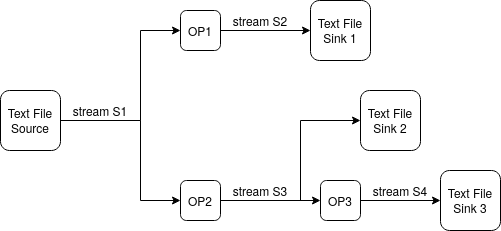
\includegraphics[scale=0.3]{./chapter3/greatSellerApp.png}}
\caption{Great Seller Dataflow Model}
\label{fig:Great Seller Dataflow Model}
\end{figure}

After developing the non-privacy-aware application, a Great Seller client specifies a View Creation Policy (VCP) on the stream number two and a Data Subject Eviction (DSEP) Policy on the stream number three.

\begin{itemize}
\item VCP: the client does not want that the employees of a market consultancy (MarketConsult employees) know if the spent amount of the client in the last 30 minutes is bigger than \euro{100} and if the number of issued transactions by the client is bigger than 3, in such case, the spent amount should be modified to the biggest allowed (\euro{100}).
\item DSEP: the client does not allow that data goes to the statistics 3 operator when MarketConsult observes the application.
\end{itemize}

After defining these specifications, the application must be modified with four elements. The first element is an observer source that provides the static context variables (SCVs). These SCVs are going to be taken into account when MarketConsult observes the application for the DSEP and when an employee of MarketConsult observes the application for the VCP. The second element that must be introduced is a Past Condition Checker (PCC) that must check if the number of issued transactions by the client in the last thirty minutes is bigger than 3. PCC is going to be connected to the third element which is the View Builder. This third element takes as inputs the output of the PCC, the stream number 3 and the observer tuple. Moreover, this element will substitute the spent amount in stream three to \euro{100} when the PCC condition is satisfied and the spent amount is bigger than \euro{100}. Finally, a Data Subject Evictor element is located on the stream three in order to remove the tuples of the client from the stream three when Market Consult is observing the application. In the figure \ref{fig:Great Seller Privacy Dataflow Model} can be seen how the application looks after applying the privacy operators.

\begin{figure}
\centering
{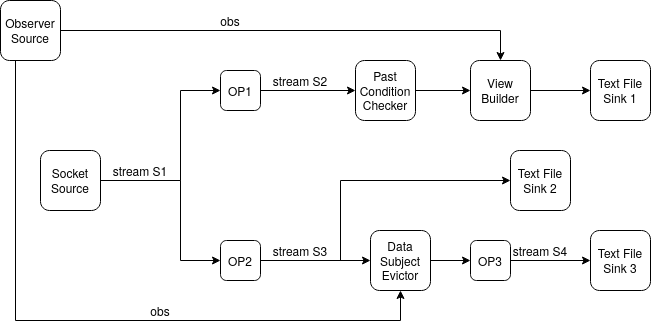
\includegraphics[scale=0.3]{./chapter3/greatSellerPriv.png}}
\caption{Great Seller Privacy Dataflow Model}
\label{fig:Great Seller Privacy Dataflow Model}
\end{figure}

All these operators can be already found in a library. However, StreamGen has not been developed to import and to generate automatically the codes of a given application working with such privacy operators.
